\subsection{Formato}
The key point for the user to understand what we want to transmit is to create a fluid communication between the representation
of the data the user. For this we must ensure that we speak the same language, with a vocabulary that is easy to understand and
with proximity, that is, leaving the terminology aside and communicating the objective in the simplest way possible.
Therefore, the representation of the information will play a fundamental role so that the
information is absorbed by the user in a natural way.


\subsubsection{How to solve it} 
This model should provide the information to the user in a compressible language or format. If it is not possible, we will provide the
necessary tools so that he can understand the context of the information.
We must study what type of representation is more appropriate, not always a graph is the most appropriate representation, we should make a
study of both the target audience and how we can accentuate the information that is most relevant in the way
correct
If we decline to make a representation with graphics, we must study the data to know what type of graph. For example,
if we talk about samples and we want to know the density, we will lean towards a density graph and if for example we look for the difference
between sexes, we will use a pie chart.

\subsubsection{How we solve it. Aire Guru} 
The Air Guru tool presents the information in the native language of the city and uses a simple and direct language.
Colors and graphic resources are used as icons. In addition, a structure has been chosen to represent the data and is repeated in disks
parts instead of creating a different visualization, so the user should only assimilate a single formula.

One of the objectives is to represent pollution by areas of the city, which is why a map has been used.
 the general AQI calculated. This is a more readable format for users since it does not have to work to make a visual image
 of the different places in the city. This index shows an indicator with five levels represented by a color scale from the
 turquoise to red ("Good" "Fair" "Poor" "Bad" and "Unhealthy"). The reason for this choice is because of the official colors and
 this avoids creating confusion for the user if he consults official sources.
 \newpage
 \begin{figure}[ht]
    \centering
    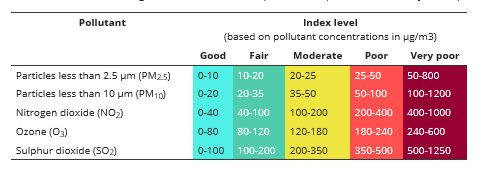
\includegraphics[width=12cm]{EAQI}
    \caption{EAQI Levels}
\end{figure}

The iconographic used to help the user to have a direct idea of the situation, since they are more
Explanatory than colors. In case of danger, it is well represented with the color red, but in the case of blue or green, in our culture, not
we have defined a state for these colors. \\
\begin{figure}[ht]
    \centering
    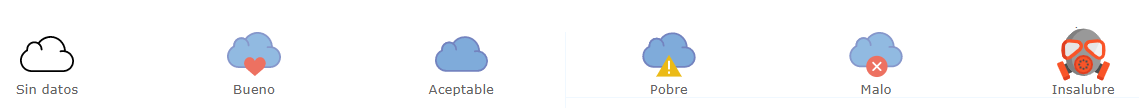
\includegraphics[width=10cm]{EAQI_Icons}
    \caption{Iconografica Aire Guru}
\end{figure}

For the graphs that show variations in time, line graphs have been used, which are the most appropriate for this type of data,
since they show the continuous evolution during a period of time. To represent the different components of the AQI, a
graph of stacked bars, since it is seen that proportion of the total AQI is formed by what pollutant. \\
\begin{figure}[ht]
    \centering
    \subfigure[AQI Evolution]
     {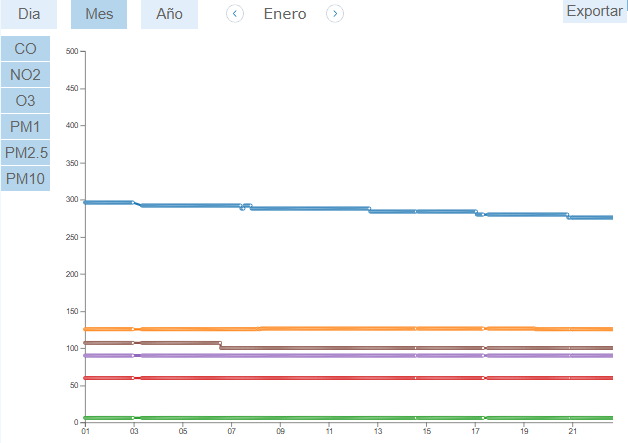
\includegraphics[width=5.75cm]{lineChart}}
     \hfill
     \subfigure [AQI components]
    { 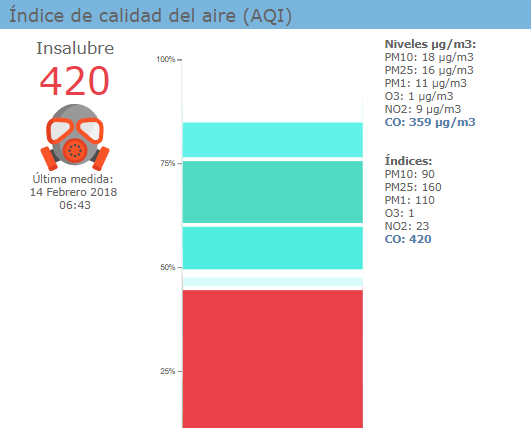
\includegraphics[width=5.25cm]{stakedBarChart}}
 
    \caption{Charts}
\end{figure}

In addition, to explain the concept of AQI and create an awarnes about the influence that air pollution has on us, Air Guru provides a
glossary and an aid with the descriptions of the polluting agents, medical complications, sources of contamination, the iconography used and
an explanation of what is and how the AQI is calculated. \\

 
\elsparagraph{Evaluation}  
\begin{itemize}
    \done The language used in the whole tool is a common language, it avoids the scientific terminology but it provides the information
         enough to understand the situation.
    \done The most appropriate graphs for each type of data have been studied and used.
    \crossed Some specific terms could not be substituted as "Air Quality Index".
    \done The necessary tools have been provided to understand the concept. The European standard of air quality has been used to
         represent the values and offer the user resources on the page for their comprehension in addition to external resources.
\end{itemize}
 

\newpage